\documentclass{standalone}
\usepackage{tikz}

\begin{document}

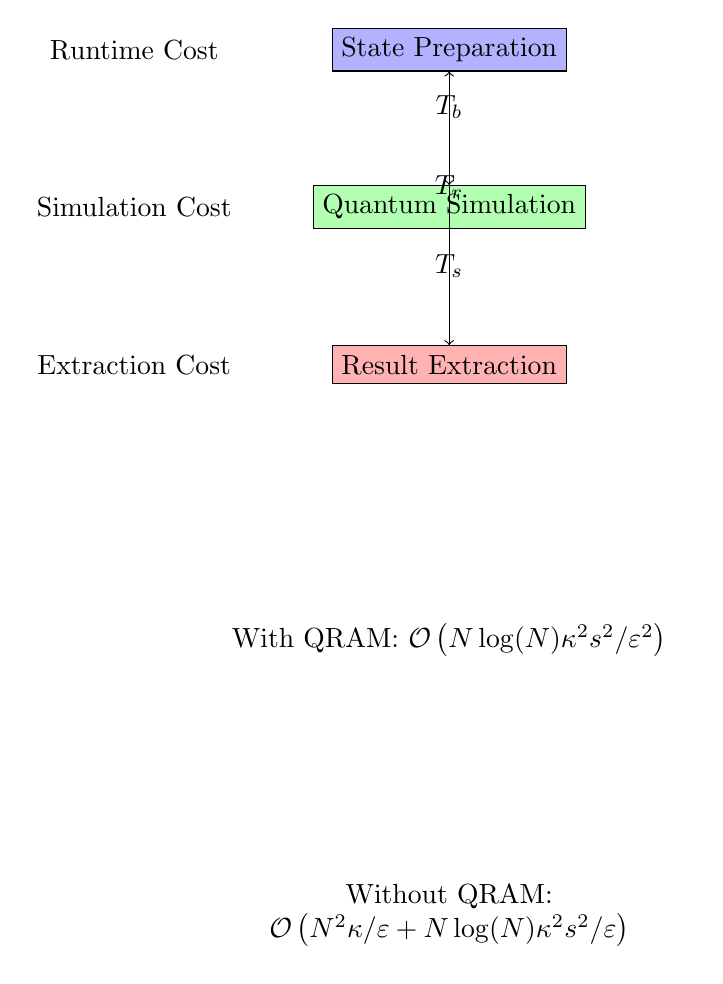
\begin{tikzpicture}[node distance=2cm]
    % Nodes
    \node (qb) [rectangle, draw, fill=blue!30] {State Preparation};
    \node (qs) [rectangle, draw, fill=green!30, below of=qb] {Quantum Simulation};
    \node (qr) [rectangle, draw, fill=red!30, below of=qs] {Result Extraction};

    % Arrows
    \draw[->] (qb) -- node[above] {$T_b$} (qs);
    \draw[->] (qs) -- node[above] {$T_s$} (qr);
    \draw[->] (qr) -- node[above] {$T_r$} (qb);

    % Complexity expressions
    \node (complexity_qram) [below of=qr, yshift=-1.5cm, text width=6cm, align=center] {
        With QRAM: $\mathcal{O}\left( N\log(N) \kappa^2 s^2 / \varepsilon^2 \right)$
    };
    \node (complexity_no_qram) [below of=complexity_qram, yshift=-1.5cm, text width=6cm, align=center] {
        Without QRAM: $\mathcal{O}\left( N^2\kappa / \varepsilon + N\log(N) \kappa^2 s^2 / \varepsilon \right)$
    };

    % Labels for components
    \node (label_qb) [left of=qb, xshift=-2cm] {Runtime Cost};
    \node (label_qs) [left of=qs, xshift=-2cm] {Simulation Cost};
    \node (label_qr) [left of=qr, xshift=-2cm] {Extraction Cost};
\end{tikzpicture}

\end{document}